% !TeX root = ../main.tex

\chapter{图像显著性检测}

\section{图像显著性检测简介}

场景中的前景对象与其背景形成明显的视觉差异时,能够快速吸引视觉注意力,称为显著区域。
人类视觉系统会自动从复杂的场景中选择性地关注显著区域,并为之分配注意资源,这被称为视觉注意机制。
有学者将这种机制引入图像分析领域,从而诞生了显著性检测(Saliency Detecion)技术,可以从海量的图像信息中快速发现关键的信息,优先分配计算资源进行处理。
显著性检测具体可分为视觉注视点预测(Visual Saliency Prediction)和显著性目标检测(Saliency Object Detecion)。
本文主要讨论的是显著性目标检测,其目的是检测和分割图像中的显著性目标,以像素级的标签标记目标的完整区域。
显著性目标检测的结果称为显著图(Saliency Map),显著图为灰度图,如图 \ref{fig:example} 所示,黑色为背景,白色为显著物体,像素的灰度值反映显著度的大小。

\begin{figure}[h]
    \centering
    \begin{subfigure}{.4\textwidth}
        \centering
        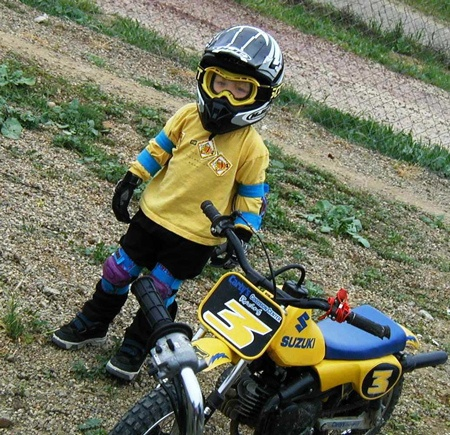
\includegraphics[width=\textwidth]{1.jpg}
        \caption{原图}
    \end{subfigure}
    \begin{subfigure}{.4\textwidth}
        \centering
        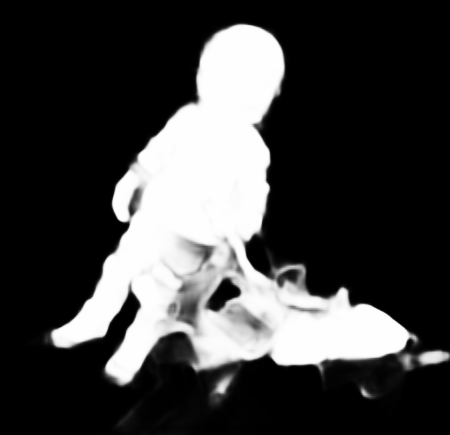
\includegraphics[width=\textwidth]{2.png}
        \caption{显著图}
    \end{subfigure}
    \caption{显著性目标检测结果示例}
    \label{fig:example}
\end{figure}

传统的具有代表性的视觉显著性目标检测算法有很多。IT\cite{IT} 算法采用自底向上的思想,将图像中各像素点在颜色、亮度、方向方面与相邻像素点的
对比值来计算显著度的大小。SR\cite{SR} 算法是基于频域分析的纯数学计算方法,无需特征提取,只需分析图像的对数频谱。
LRMR\cite{LRMR} 算法将图像分为稀疏矩阵(显著区域)和低秩矩阵(背景区域),图像经过稳健主元分析技术进行低秩矩阵恢复算法,
差异部分得到的即为显著区域。然而,由于缺乏高级语义信息,导致这些算法在复杂场景难以有效实现前景目标和背景图像的分离。

近年来,随着机器学习的强势崛起,越来越多的致力于显著性目标检测的学者开始把目光投向深度学习,并取得了瞩目的成果。
深度神经网络的结构采用端到端的方式,分为多层,上一层的输出直接作为下一层的输入,每层为卷积,池化或非线性激活函数
ReLU\footnote{\url{https://pytorch.org/docs/stable/generated/torch.nn.ReLU.html}}。
经过数据集训练后,可以自适应地
提取高级语义特征,从而克服人工提取特征的局限性。当前基于深度学习的显著性目标检测面临到两个问题,一是如何融合多层次深度特征,二是显著性物体的边界质量
容易受到损失函数的影响。学者们纷纷致力于探索更加有效的神经网络结构以解决这些问题。
BASNet\cite{BASNet}使用一个编码-解码网络(即U型网络)进行显著性预测,再通过一个精心设计的残差模块来细化预测边界。AFNet\cite{AFNet}在U型网络
的基础上,在每层都嵌入了注意力反馈模块,并采用边界强化损失作为损失函数。PoolNet\cite{PoolNet}在U型网络的基础上提出全局引导模块和特征整合模块
控制多级特征图与高级特征语义无缝融合。

\section{PoolNet简介}

如图 \ref{fig:net} 所示,论文依旧使用U型网络,但在此基础上提出了两个亮眼的模块:
一是全局引导模块(GGM),目的是为不同特征级别的特征图提供高级语义信息。
二是特征整合模块(FAM),目的是使粗略高级语义信息与上采样路径中的细微特征无缝融合。
由于这两个模块均是依赖于池化技巧,因此命名为PoolNet。
下面将围绕U型网络,全局引导模块和特征整合模块三个方面展开介绍。

\begin{figure}[h]
\centering
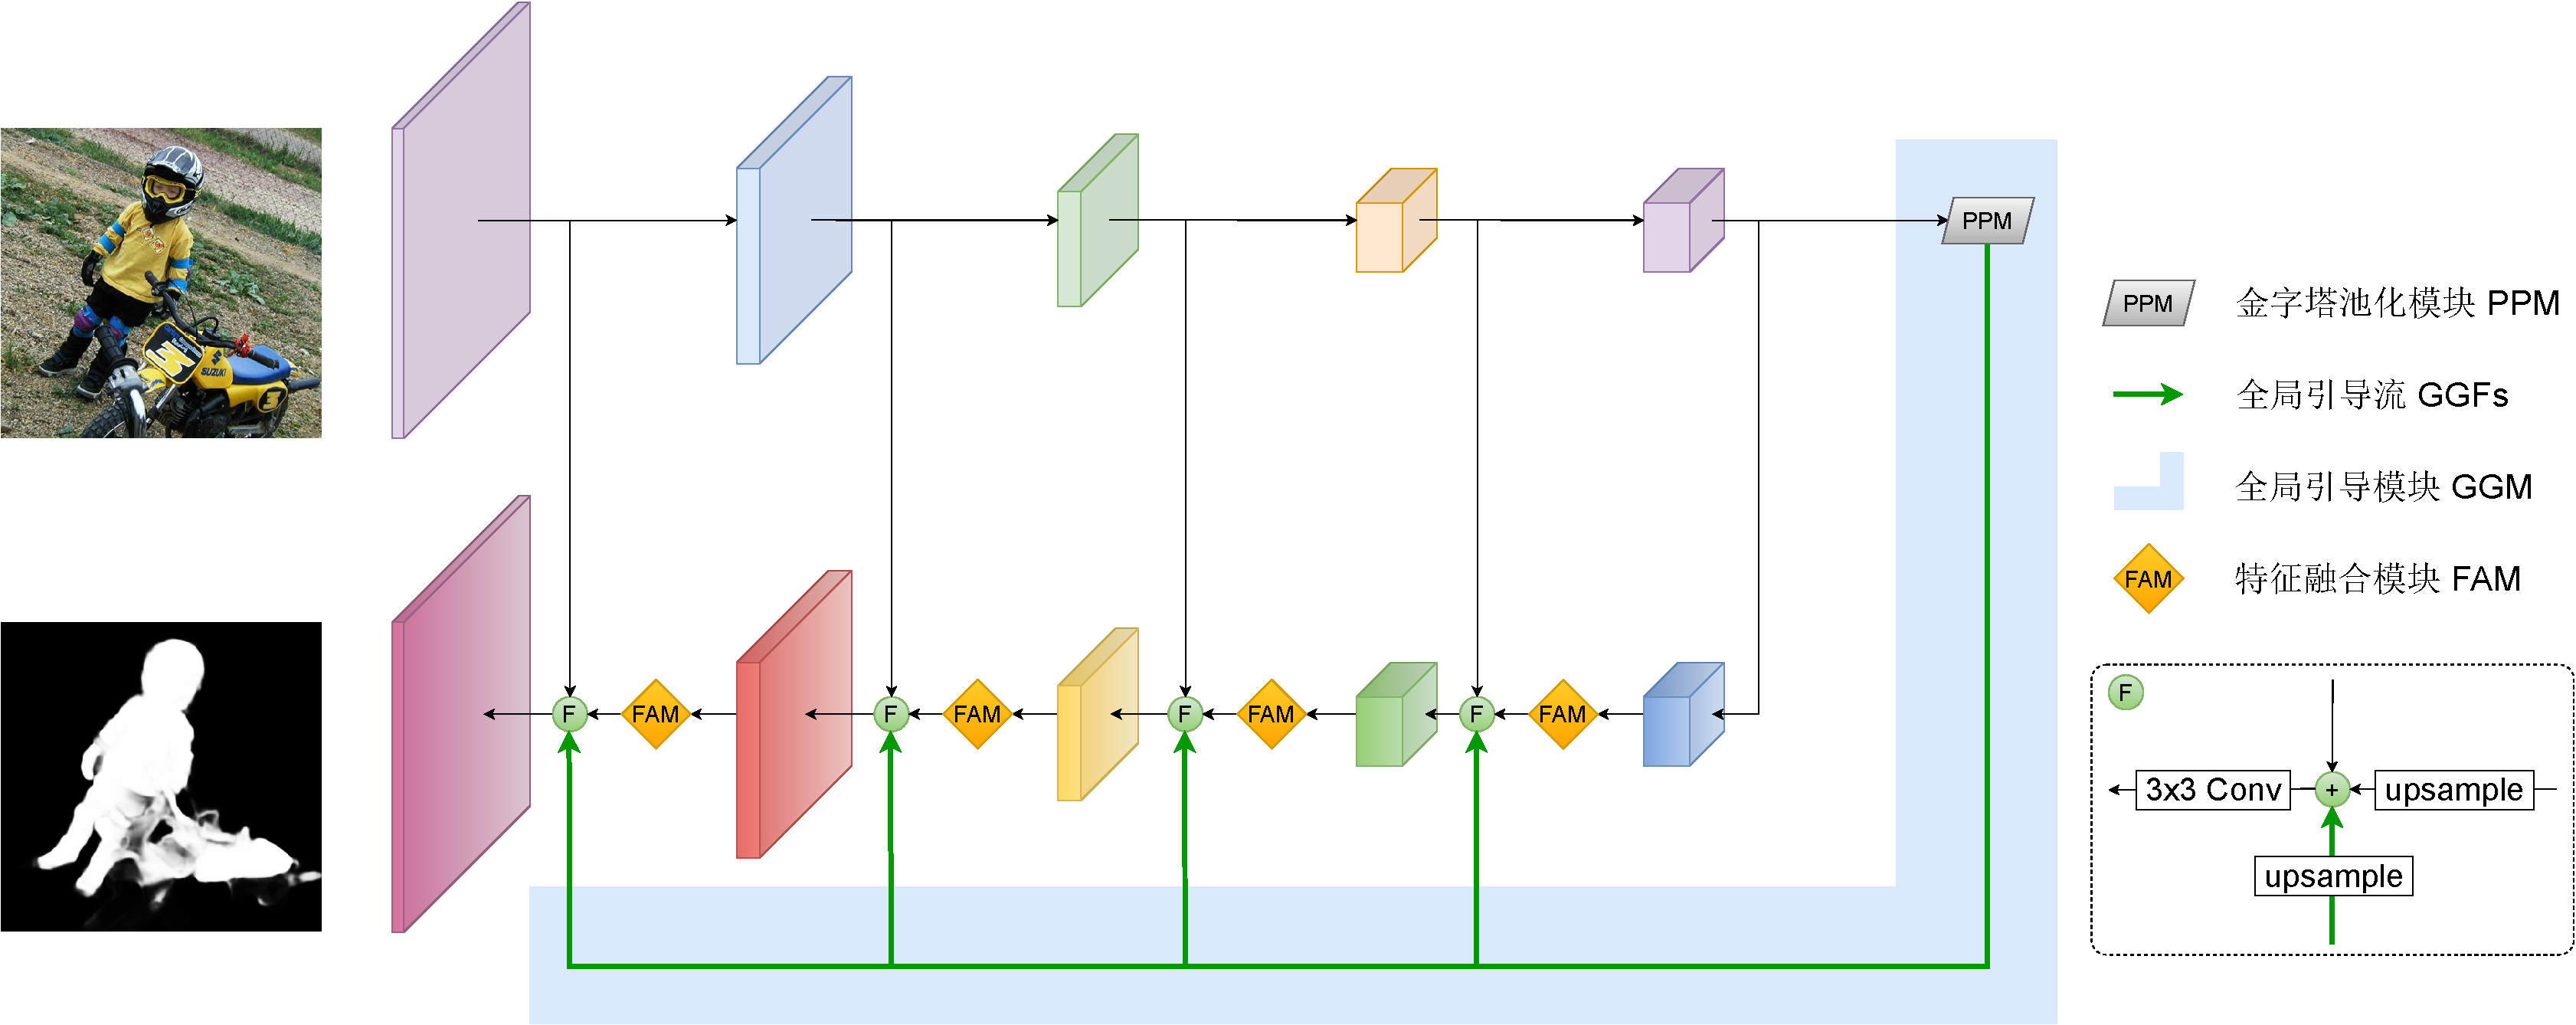
\includegraphics[width=1\textwidth]{poolnet.pdf}
\caption{PoolNet 整体架构}
\label{fig:net}
% \note{注:图注的内容不宜放到图题中。}
\end{figure}

\subsection{U型网络}

U型网络,又称编码器-解码器网络,最早由Olaf Ronneberger\cite{U-Net}等人提出并应用于医学图像分割。U型网络是一种语义分割网络,包含了
一个用于提取高层语义信息的收缩网络和一个用于输出定位的上采样网络,来自收缩网络中的高分辨率特征与上采样输出相结合,可以使定位更加精确。
该网络在少量数据训练的情况下可以获得精确的分割结果。

PoolNet 继续沿用了U型网络,收缩网络使用经典架构 deeplab\_resnet50\cite{deeplab}\cite{resnet},上采样网络使用双线性插值,以尺寸为300x400的3通道图片作为输入,
中间特征图的变化如图 \ref{fig:UNet} 所示。

\begin{figure}[h]
\centering
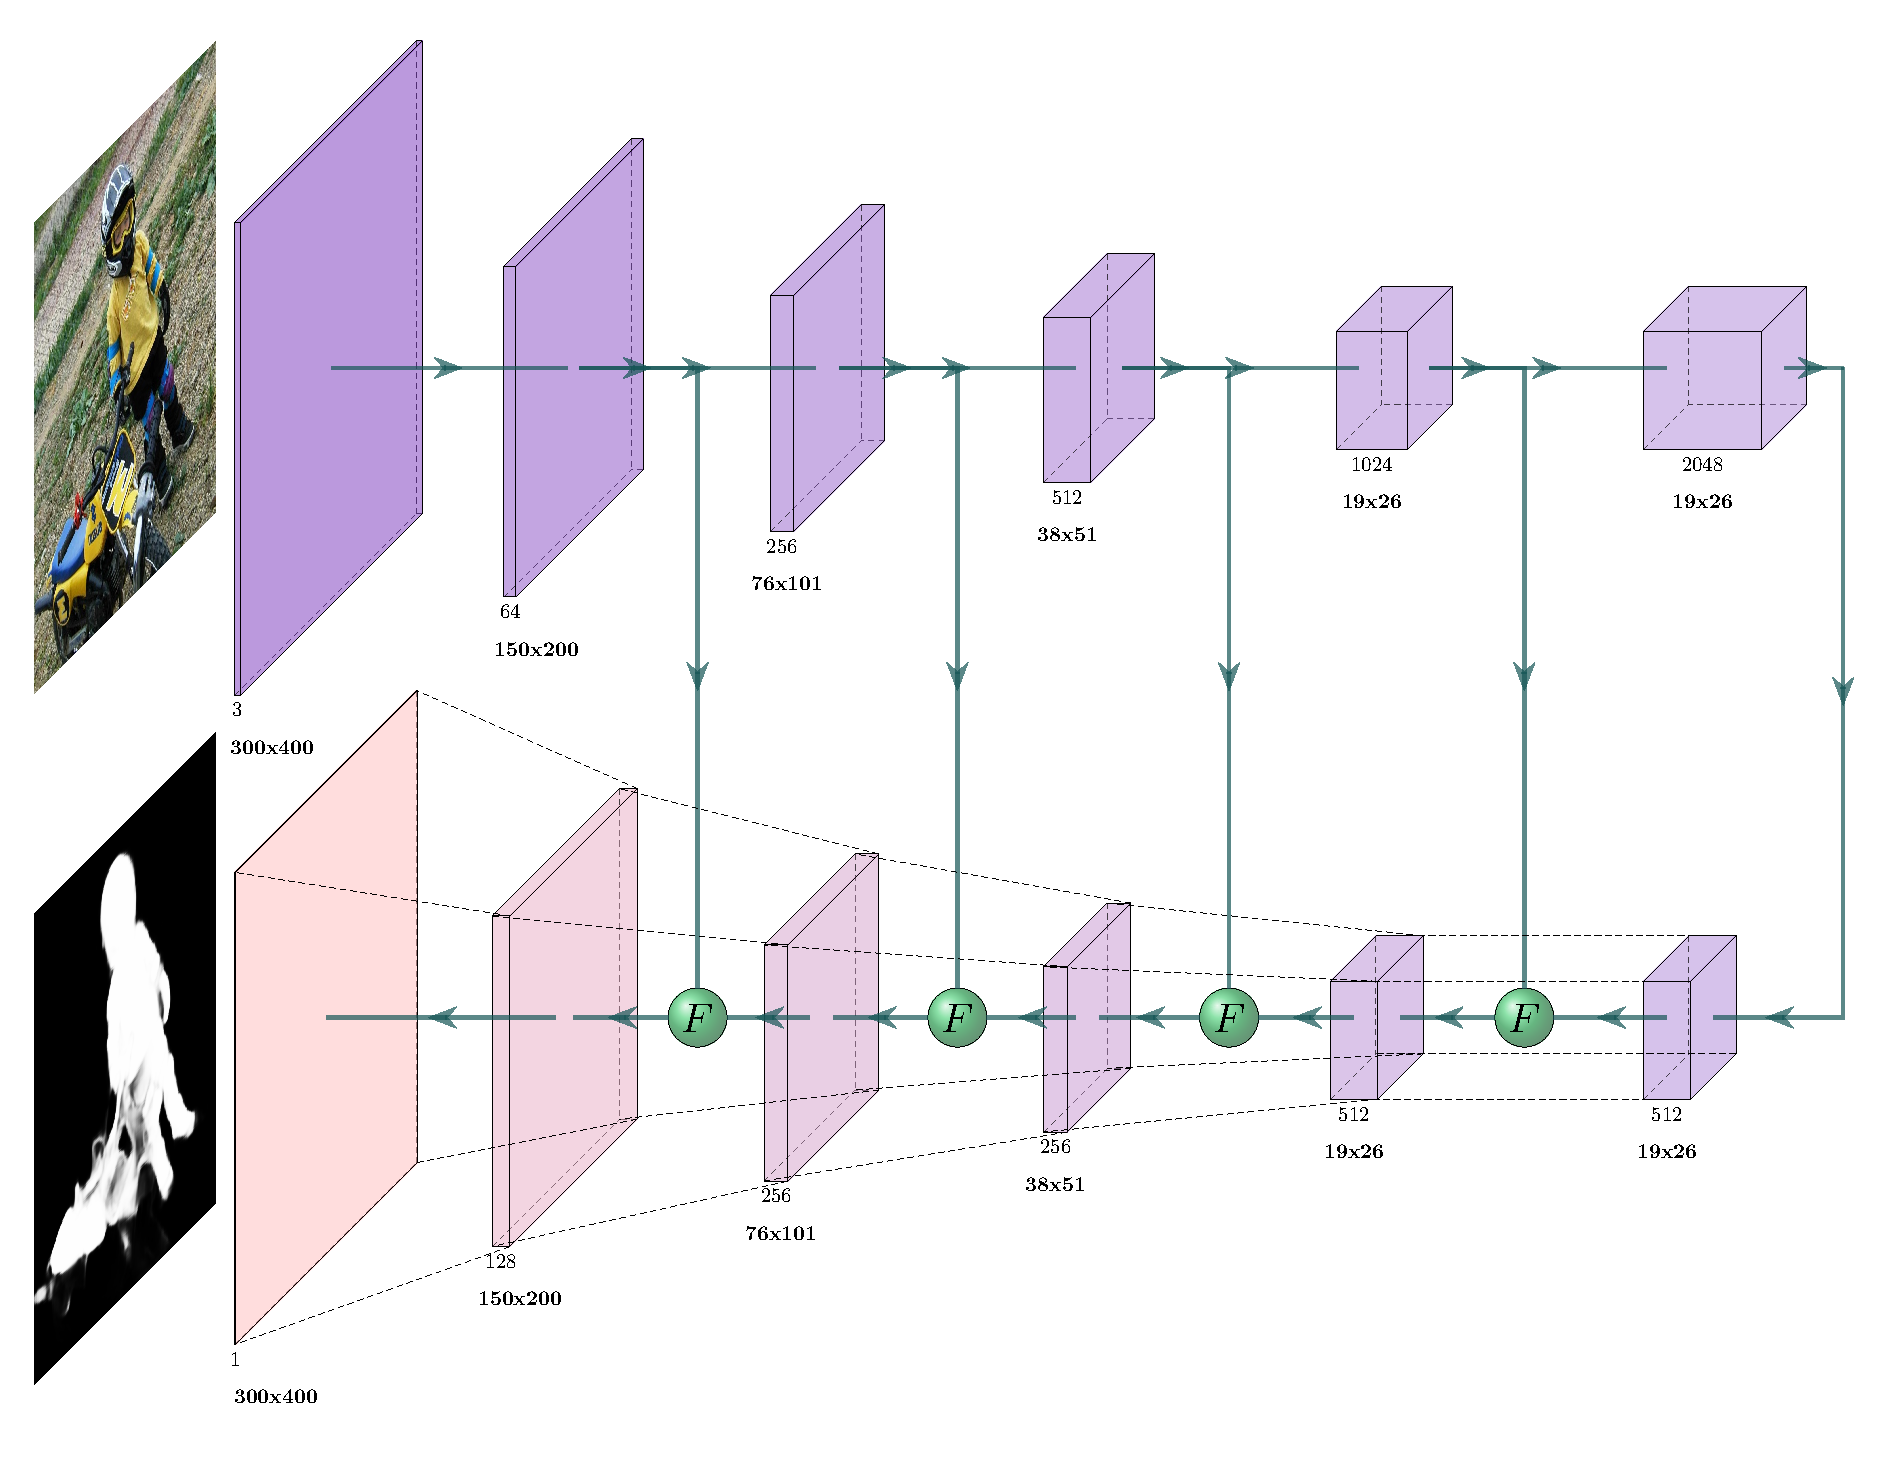
\includegraphics[width=1\textwidth]{UNet.pdf}
\caption{U型网络}
\label{fig:UNet}
% \note{注:图注的内容不宜放到图题中。}
\end{figure}

尽管U型网络取得了很好的效果,但是依旧存在很大的提升空间。首先,在上采样过程中,U型网络底层获得的高级语义信息不断向上层传播,导致逐渐被
稀释。其次,正如Zhao\cite{Zhao}等人指出的那样,CNN 网络的感受野并非和网络的深度成比例关系。针对这两个问题,PoolNet 提出了GGM和FAM模块

\subsection{全局引导模块(GGM)}

高层语义特征对定位显著物体的具体位置有很大作用,但是网络骨架获得的高级语义信息在上采样过程中会不断被稀释,导致其产生的作用会被限制。
除此之外,在实际的实验中\cite{Zhao}\cite{Zhou},CNNs 网络的感受野比理论值要小得多,这一点对于深层网络非常明显,导致网络难以捕捉全局信息。考虑到对于上采样
过程中高级语义信息的缺失,PooNet 引入了全局引导模块GGM,包含了一个改进的金字塔池化模块PPM和一系列全局引导流GGFs,目的是为了使每一级
的特征图获得显著物体的位置信息。

\subsubsection{金字塔池化模块(PPM)}

该 PPM 模块融合了 4 种不同尺度的特征图。以 300x400 的输入尺寸为例,通过 backbone 得到 19x26 的特征图(图 \ref{fig:ppm} 左边蓝色块),这是尺度最大的特征。
该特征图通过 AdaptiveAvgPool2d\footnote{\url{https://pytorch.org/docs/stable/generated/torch.nn.AdaptiveAvgPool2d.html}}
分别池化为 1x1,3x3,5x5 三种小尺寸特征,经过卷积层后,再经过上采样将尺寸变回 19x26。然后将这4种特征 concat 到一起,由于通道数会变为
原来的4倍,所以还要通过一个卷积层恢复至原通道数。

\begin{figure}[h]
\centering
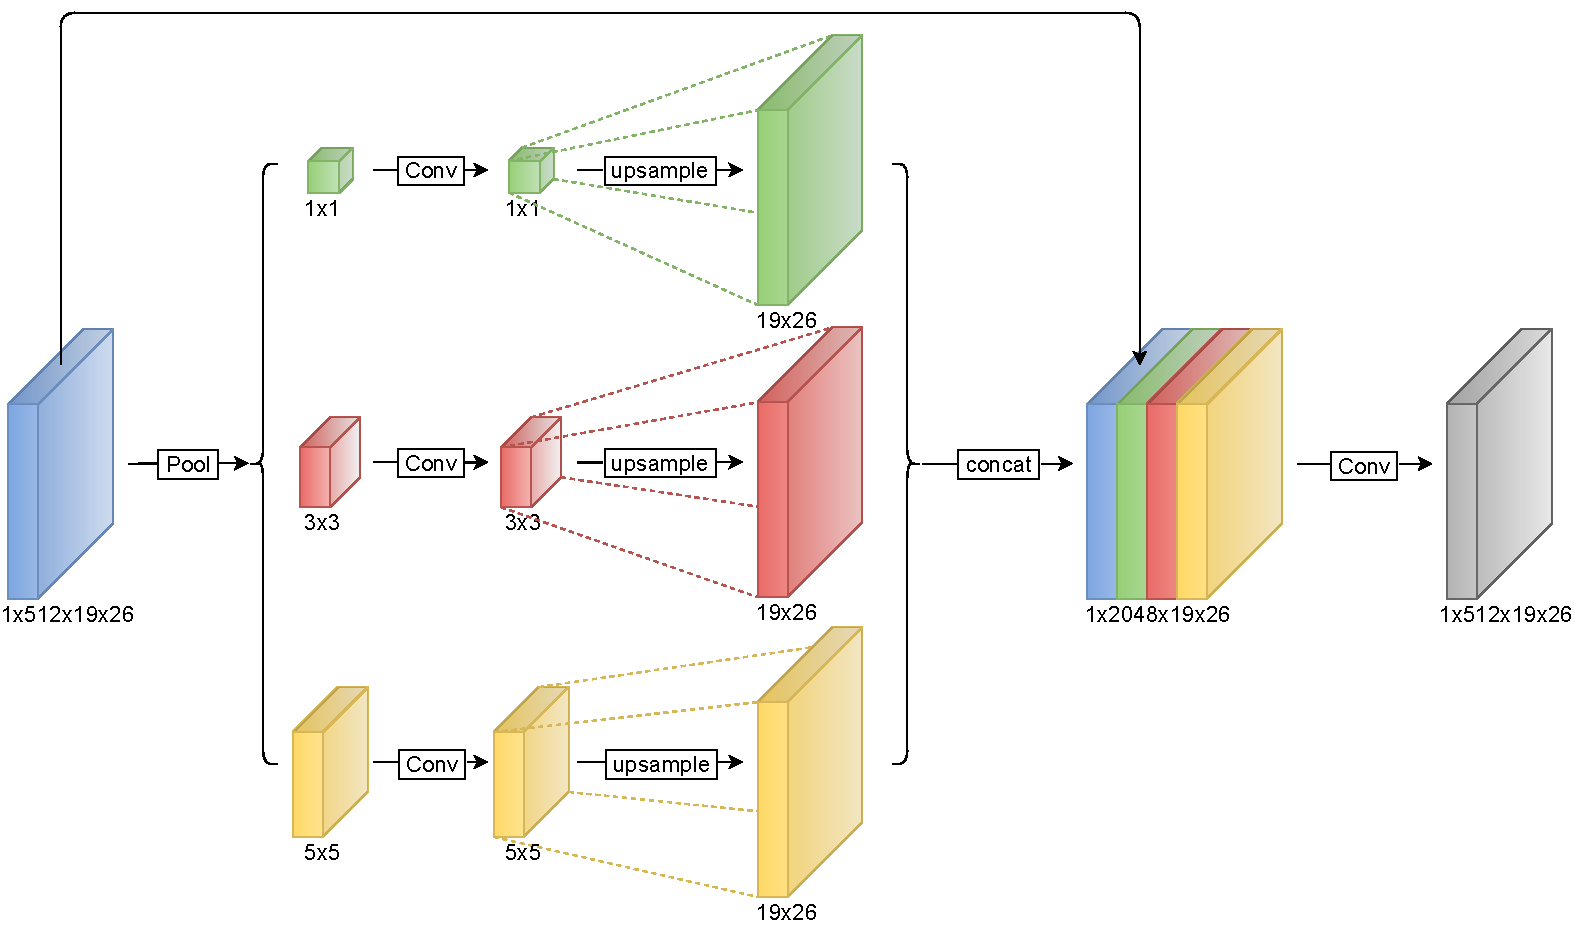
\includegraphics[width=1\textwidth]{ppm_bold.pdf}
\caption{金字塔池化模块(PPM)}
\label{fig:ppm}
% \note{注:图注的内容不宜放到图题中。}
\end{figure}

\subsubsection{全局引导流(GGFs)}

现在需要做的是思考从 PPM 模块获得的高层语义信息(图 \ref{fig:ggf} 右上角灰色块)如何融入到上采样过程不同级别的特征图中。
首先,将高级语义信息特征图分别进行比例为1,2、4、8的上采样,把尺寸调整为 19x26,38x51,76x101,150x200,对应了不同级别特征图的尺寸;
然后分别通过卷积层把通道数分别调整为512,256,256,128,对应了不同级别特征图的通道。
现在,可以进行融合了!图 \ref{fig:ggf} 中自下而上箭头部分表示在不同级别的特征图中加入高层语义信息。

\begin{figure}[h]
\centering
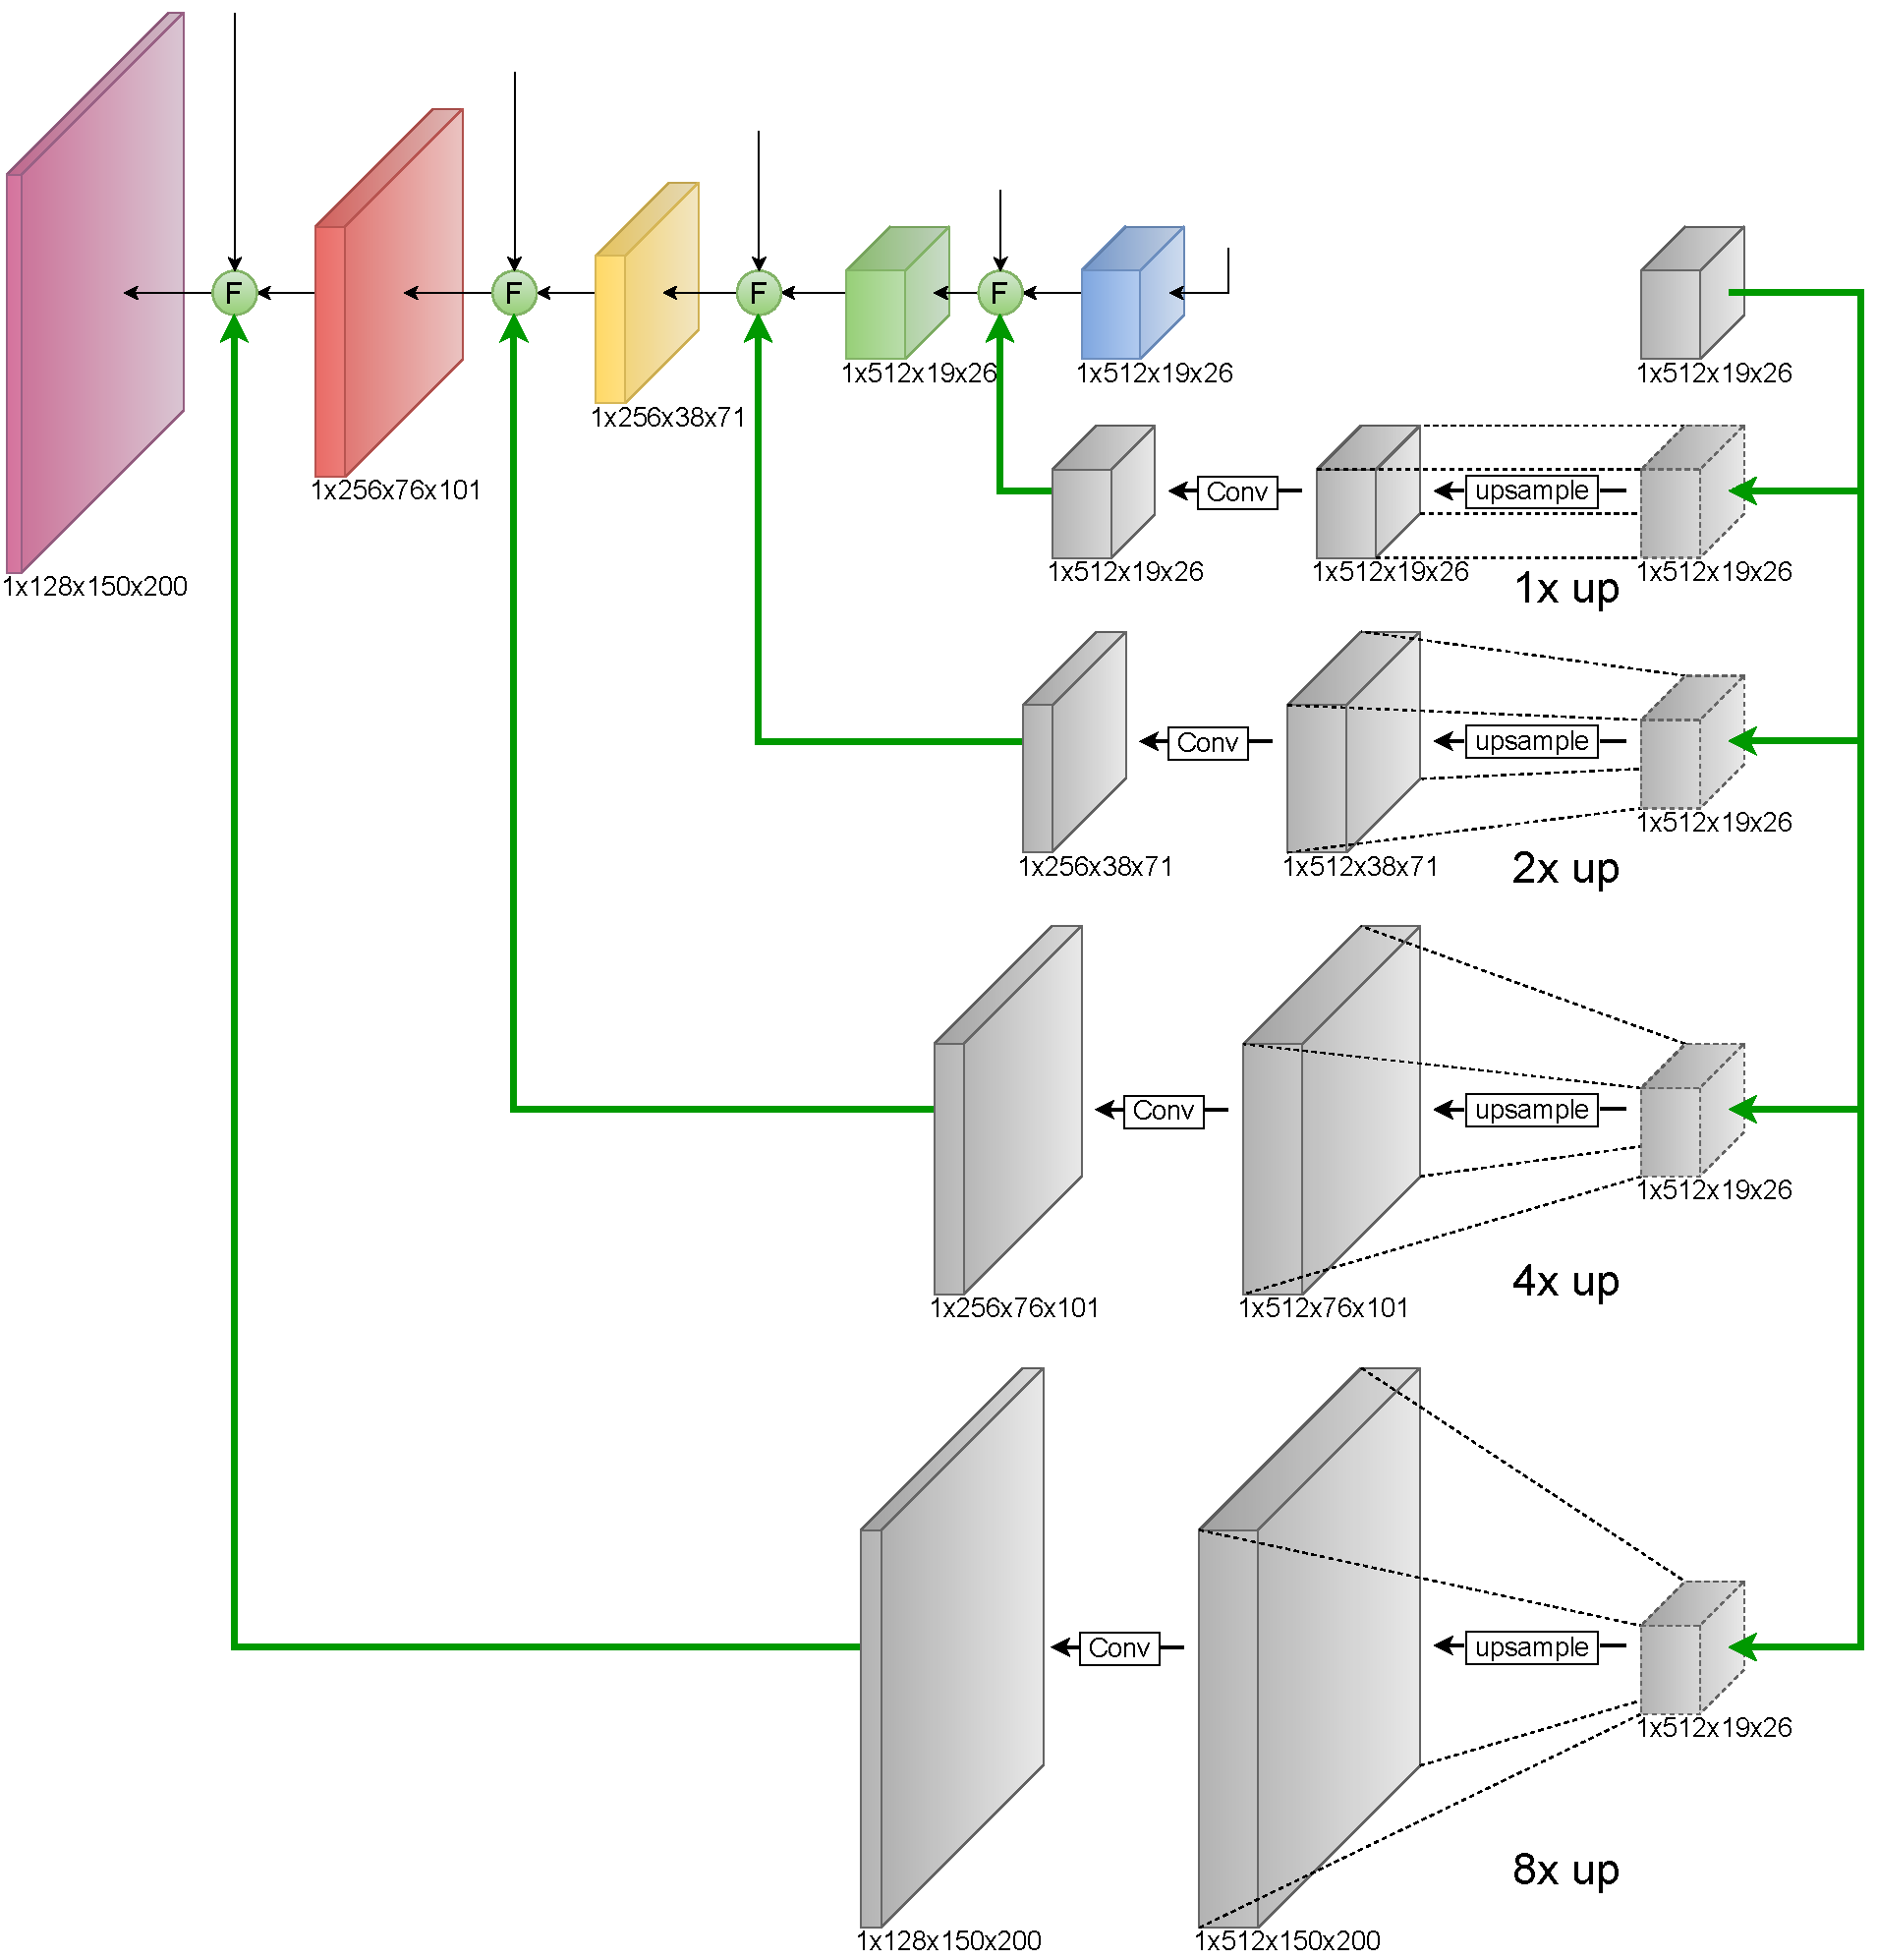
\includegraphics[width=1\textwidth]{ggfs.pdf}
\caption{全局引导流(GGFs)}
\label{fig:ggf}
% \note{注:图注的内容不宜放到图题中。}
\end{figure}

\subsection{特征整合模块(FAM)}

前面提到的 GGM 模块是在不同级别的特征图中加入高级语义信息,那么新的问题是如何使来自GGM模块的粗糙的高层语义信息和不同尺度的特征图无缝融合?
在传统的U型网络上采样过程中,相邻特征图间放缩的比例为2,与来自收缩网络各层的中低级语义信息融合后,再通过一个3x3卷积层可以很好地降低上采样
带来的混叠效应。但是,GGFs 模块为了使高层语义信息的尺寸和特征图相同,采用了较大比例的上采样(4倍,8倍),这很容易导致高级语义信息和特征图
之间产生难以逾越的鸿沟。

为了解决这个问题,PoolNet 提出了特征整合模块(FAM)。如图 \ref{fig:fam} 所示,FAM 模块包含 4 个分支,输入特征图首先经过
AvgPool2d\footnote{\url{https://pytorch.org/docs/stable/generated/torch.nn.AvgPool2d.html}}
按照 2,4,8 三种比例进行下采样,经过3x3卷积层后,再经过对应比例的上采样(双线性插值)恢复到原尺寸。
然后,这 4 个分支直接相加,再经过3x3卷积层后就做好了与高级语义信息融合的准备。

\begin{figure}[h]
\centering
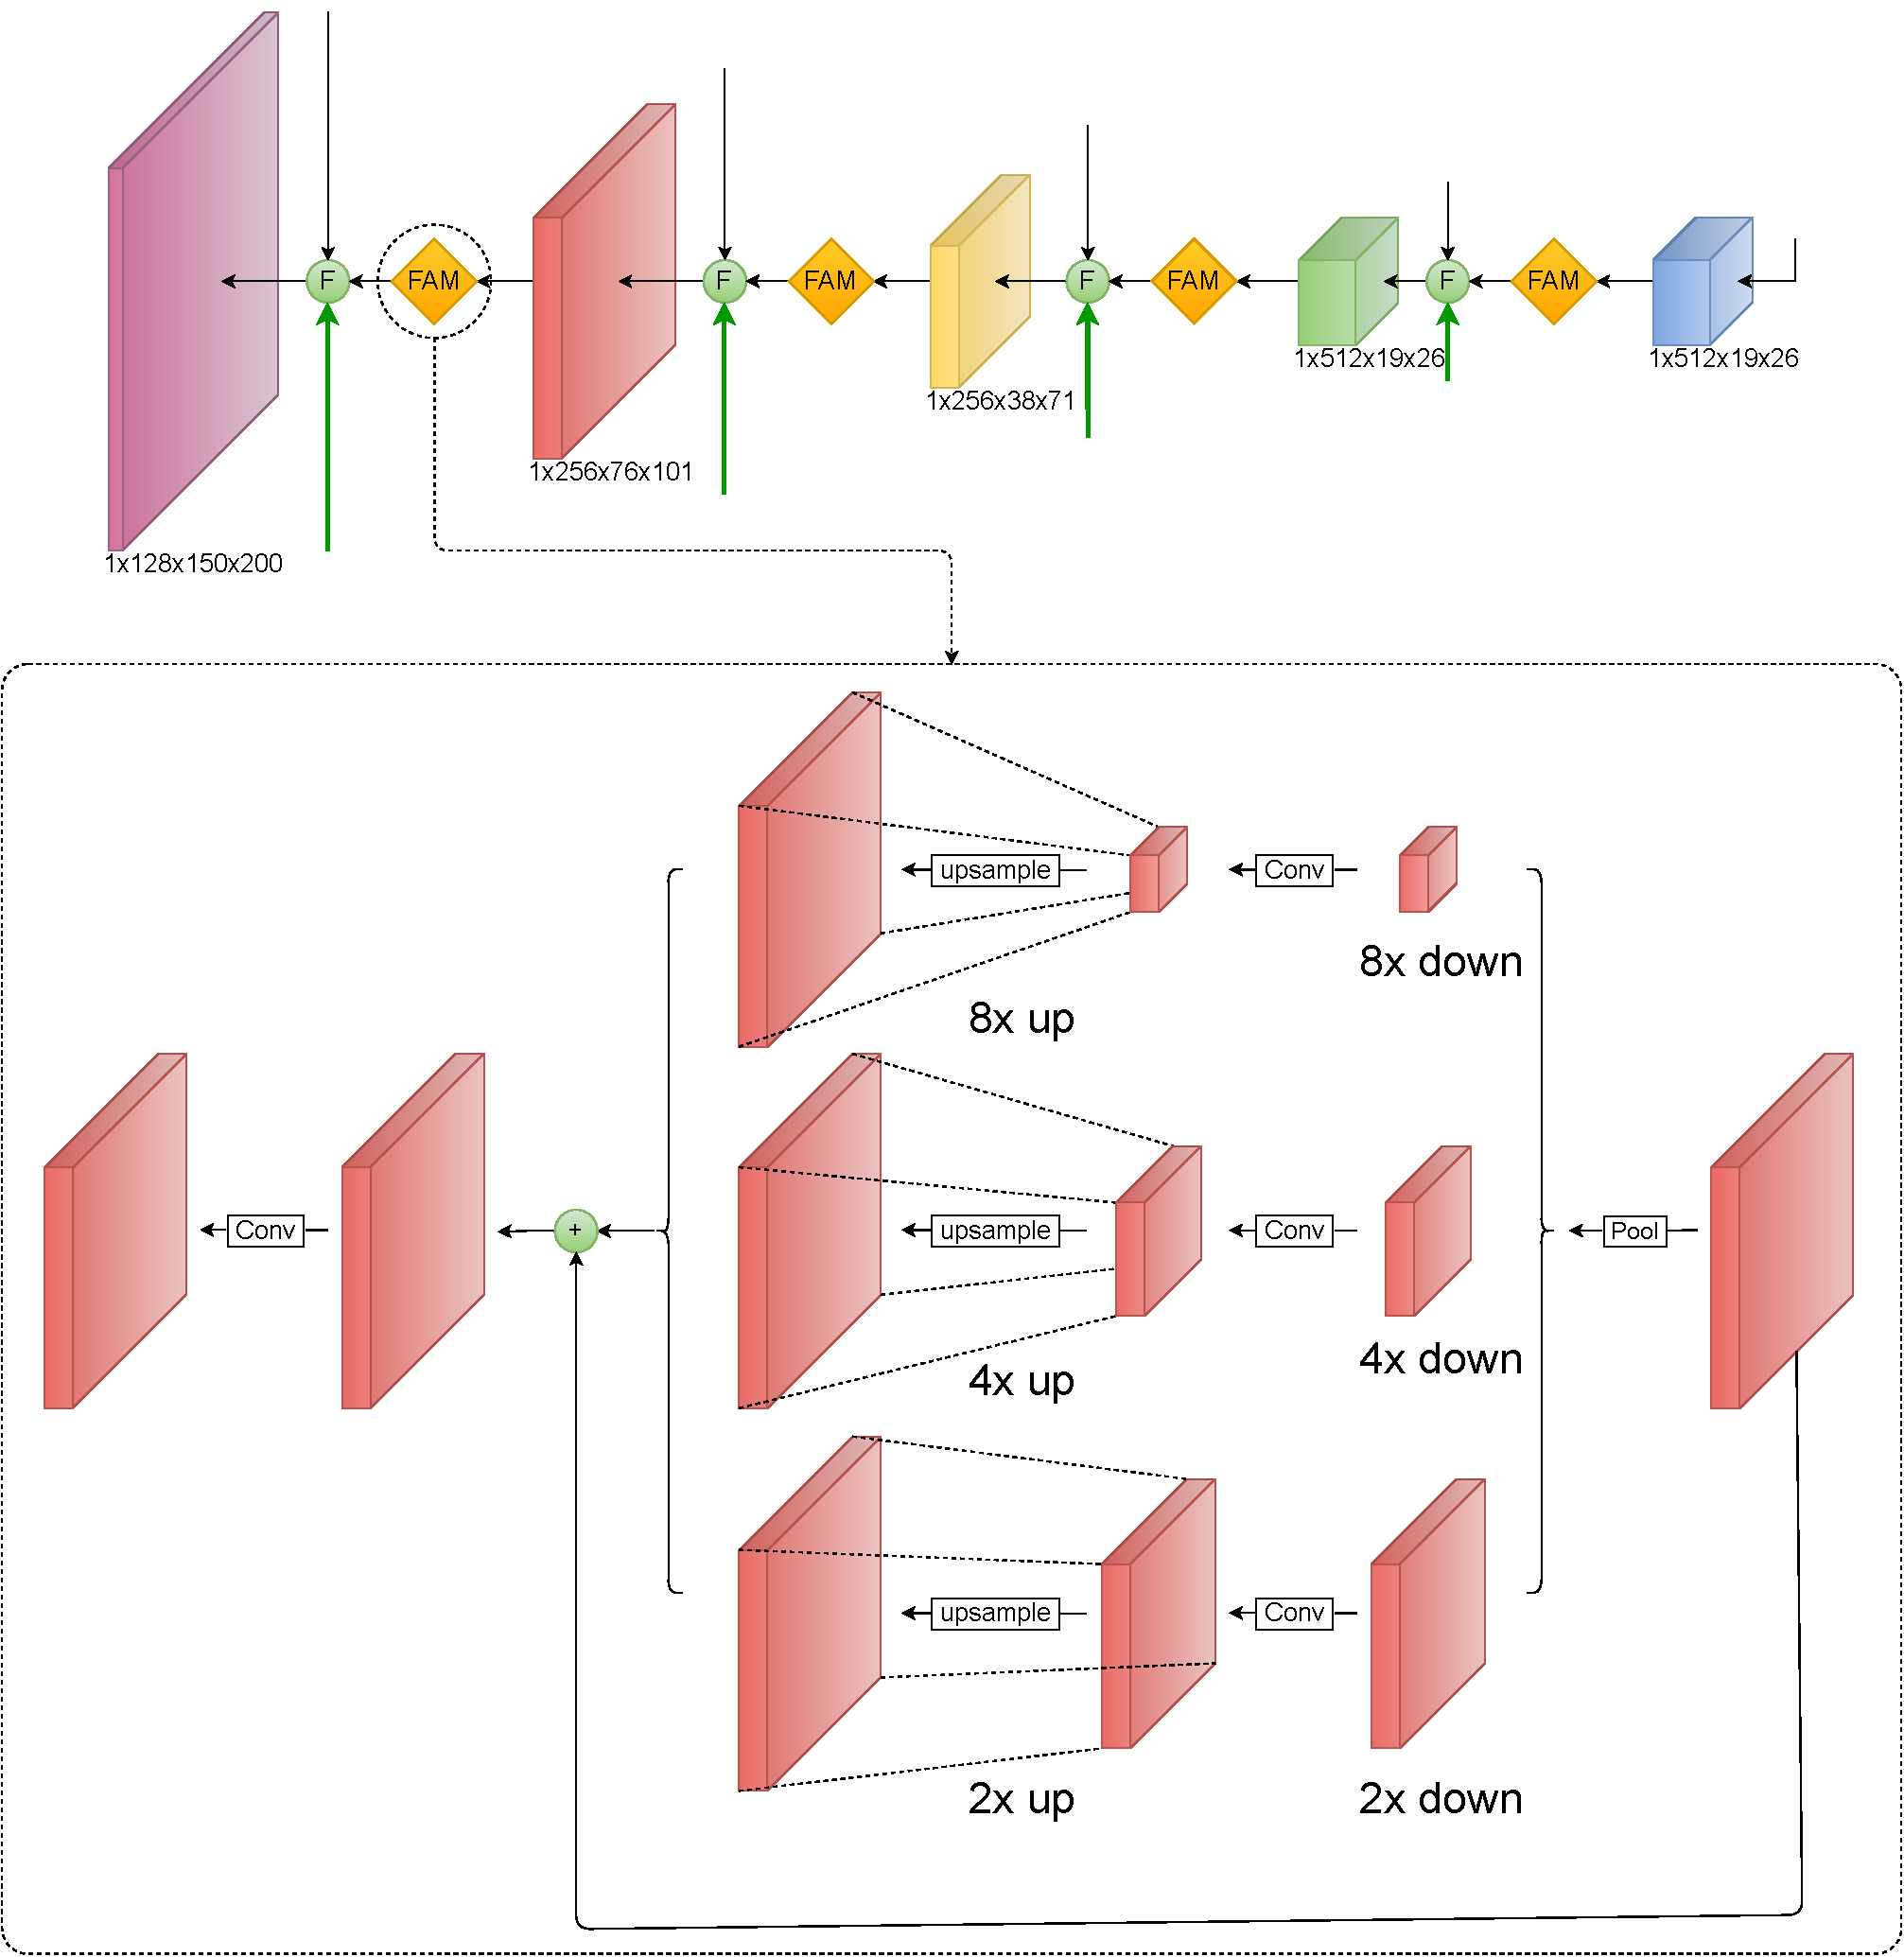
\includegraphics[width=1\textwidth]{fam.pdf}
\caption{特征整合模块(FAM)}
\label{fig:fam}
% \note{注:图注的内容不宜放到图题中。}
\end{figure}

总的来说,FAM 的作用有两点。
一是帮助模型降低了上采样导致的混叠效应,尤其是当上采样比例较大时(如4倍,8倍)。
二是从不同尺度上刻画显著物体的空间位置,增加了整个网络的感受野。
